\documentclass[1p]{elsarticle_modified}
%\bibliographystyle{elsarticle-num}

%\usepackage[colorlinks]{hyperref}
%\usepackage{abbrmath_seonhwa} %\Abb, \Ascr, \Acal ,\Abf, \Afrak
\usepackage{amsfonts}
\usepackage{amssymb}
\usepackage{amsmath}
\usepackage{amsthm}
\usepackage{scalefnt}
\usepackage{amsbsy}
\usepackage{kotex}
\usepackage{caption}
\usepackage{subfig}
\usepackage{color}
\usepackage{graphicx}
\usepackage{xcolor} %% white, black, red, green, blue, cyan, magenta, yellow
\usepackage{float}
\usepackage{setspace}
\usepackage{hyperref}

\usepackage{tikz}
\usetikzlibrary{arrows}

\usepackage{multirow}
\usepackage{array} % fixed length table
\usepackage{hhline}

%%%%%%%%%%%%%%%%%%%%%
\makeatletter
\renewcommand*\env@matrix[1][\arraystretch]{%
	\edef\arraystretch{#1}%
	\hskip -\arraycolsep
	\let\@ifnextchar\new@ifnextchar
	\array{*\c@MaxMatrixCols c}}
\makeatother %https://tex.stackexchange.com/questions/14071/how-can-i-increase-the-line-spacing-in-a-matrix
%%%%%%%%%%%%%%%

\usepackage[normalem]{ulem}

\newcommand{\msout}[1]{\ifmmode\text{\sout{\ensuremath{#1}}}\else\sout{#1}\fi}
%SOURCE: \msout is \stkout macro in https://tex.stackexchange.com/questions/20609/strikeout-in-math-mode

\newcommand{\cancel}[1]{
	\ifmmode
	{\color{red}\msout{#1}}
	\else
	{\color{red}\sout{#1}}
	\fi
}

\newcommand{\add}[1]{
	{\color{blue}\uwave{#1}}
}

\newcommand{\replace}[2]{
	\ifmmode
	{\color{red}\msout{#1}}{\color{blue}\uwave{#2}}
	\else
	{\color{red}\sout{#1}}{\color{blue}\uwave{#2}}
	\fi
}

\newcommand{\Sol}{\mathcal{S}} %segment
\newcommand{\D}{D} %diagram
\newcommand{\A}{\mathcal{A}} %arc


%%%%%%%%%%%%%%%%%%%%%%%%%%%%%5 test

\def\sl{\operatorname{\textup{SL}}(2,\Cbb)}
\def\psl{\operatorname{\textup{PSL}}(2,\Cbb)}
\def\quan{\mkern 1mu \triangleright \mkern 1mu}

\theoremstyle{definition}
\newtheorem{thm}{Theorem}[section]
\newtheorem{prop}[thm]{Proposition}
\newtheorem{lem}[thm]{Lemma}
\newtheorem{ques}[thm]{Question}
\newtheorem{cor}[thm]{Corollary}
\newtheorem{defn}[thm]{Definition}
\newtheorem{exam}[thm]{Example}
\newtheorem{rmk}[thm]{Remark}
\newtheorem{alg}[thm]{Algorithm}

\newcommand{\I}{\sqrt{-1}}
\begin{document}

%\begin{frontmatter}
%
%\title{Boundary parabolic representations of knots up to 8 crossings}
%
%%% Group authors per affiliation:
%\author{Yunhi Cho} 
%\address{Department of Mathematics, University of Seoul, Seoul, Korea}
%\ead{yhcho@uos.ac.kr}
%
%
%\author{Seonhwa Kim} %\fnref{s_kim}}
%\address{Center for Geometry and Physics, Institute for Basic Science, Pohang, 37673, Korea}
%\ead{ryeona17@ibs.re.kr}
%
%\author{Hyuk Kim}
%\address{Department of Mathematical Sciences, Seoul National University, Seoul 08826, Korea}
%\ead{hyukkim@snu.ac.kr}
%
%\author{Seokbeom Yoon}
%\address{Department of Mathematical Sciences, Seoul National University, Seoul, 08826,  Korea}
%\ead{sbyoon15@snu.ac.kr}
%
%\begin{abstract}
%We find all boundary parabolic representation of knots up to 8 crossings.
%
%\end{abstract}
%\begin{keyword}
%    \MSC[2010] 57M25 
%\end{keyword}
%
%\end{frontmatter}

%\linenumbers
%\tableofcontents
%
\newcommand\colored[1]{\textcolor{white}{\rule[-0.35ex]{0.8em}{1.4ex}}\kern-0.8em\color{red} #1}%
%\newcommand\colored[1]{\textcolor{white}{ #1}\kern-2.17ex	\textcolor{white}{ #1}\kern-1.81ex	\textcolor{white}{ #1}\kern-2.15ex\color{red}#1	}

{\Large $\underline{12n_{0352}~(K12n_{0352})}$}

\setlength{\tabcolsep}{10pt}
\renewcommand{\arraystretch}{1.6}
\vspace{1cm}\begin{tabular}{m{100pt}>{\centering\arraybackslash}m{274pt}}
\multirow{5}{120pt}{
	\centering
	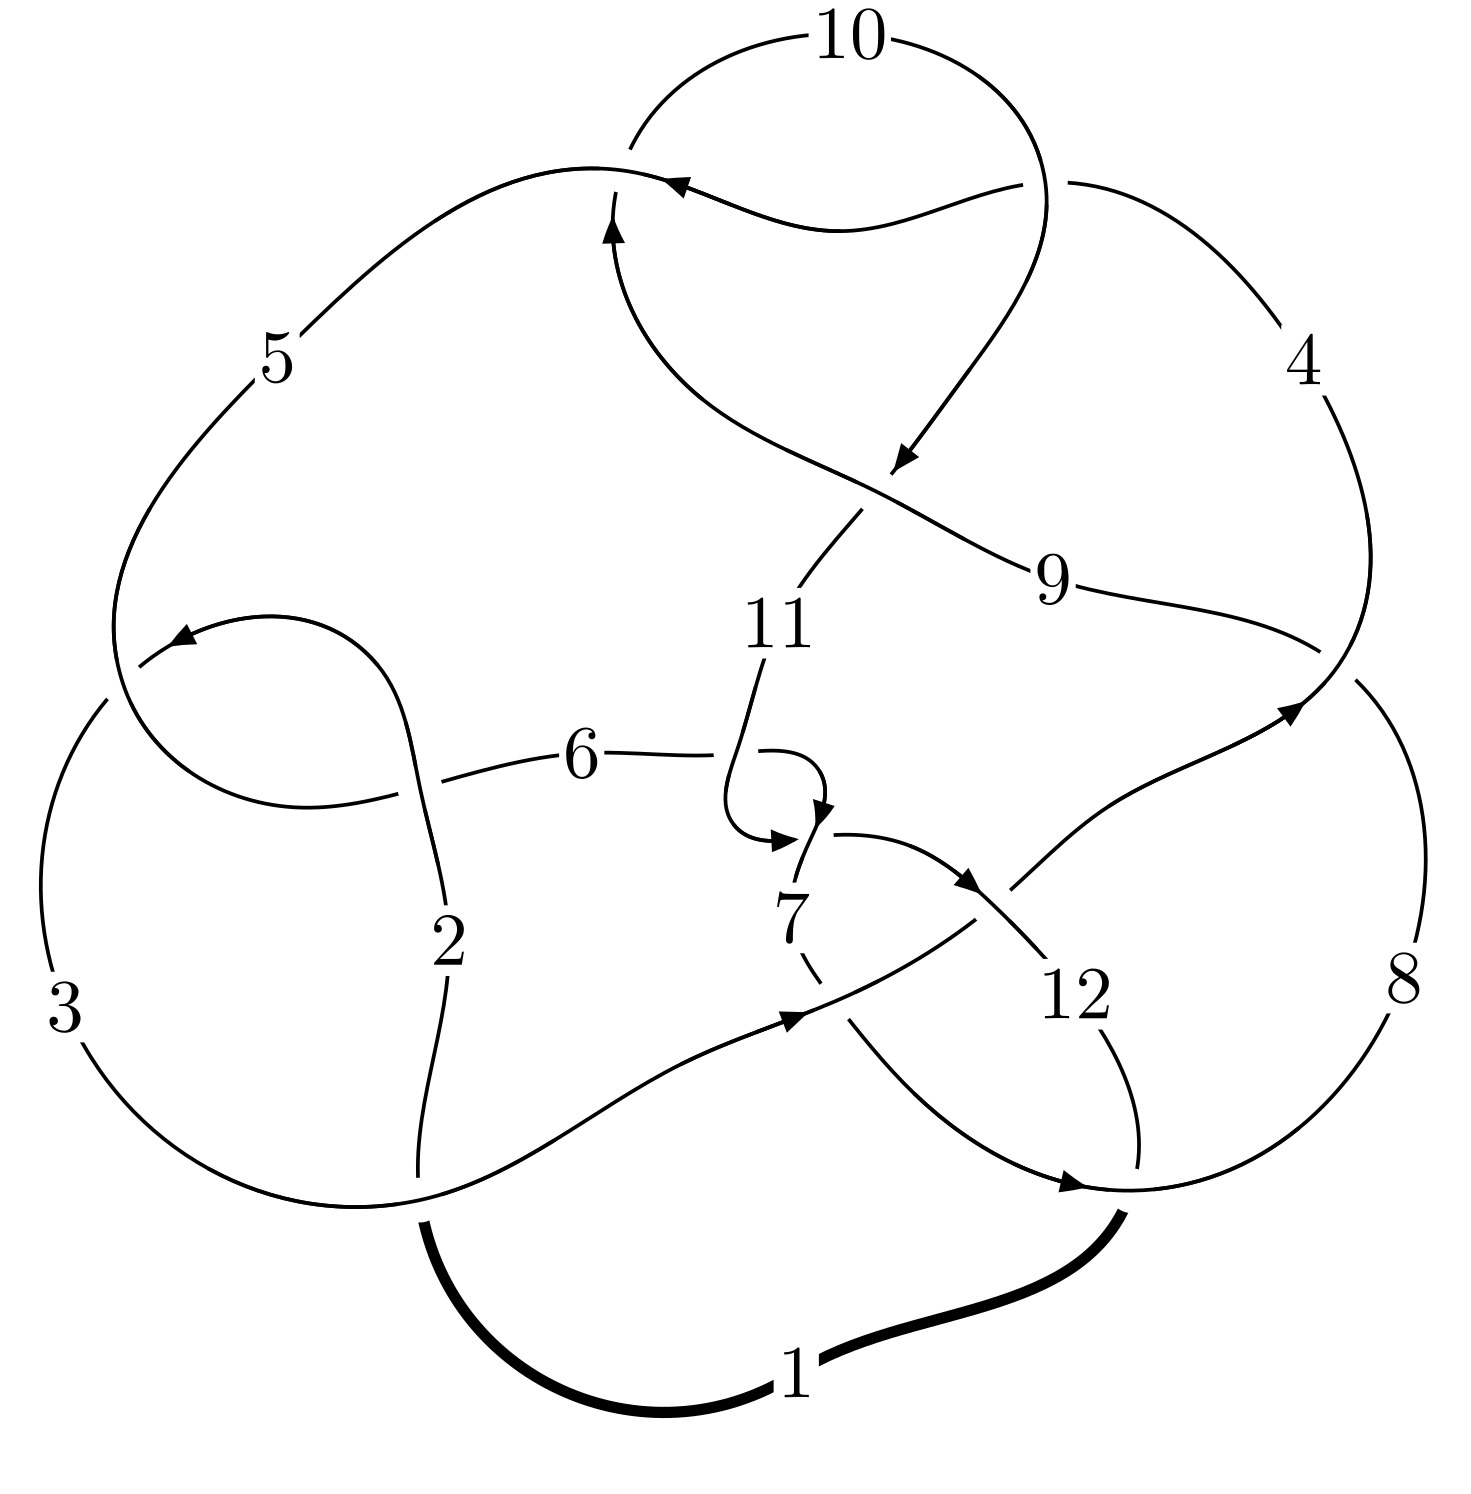
\includegraphics[width=112pt]{../../../GIT/diagram.site/Diagrams/png/2441_12n_0352.png}\\
\ \ \ A knot diagram\footnotemark}&
\allowdisplaybreaks
\textbf{Linearized knot diagam} \\
\cline{2-2}
 &
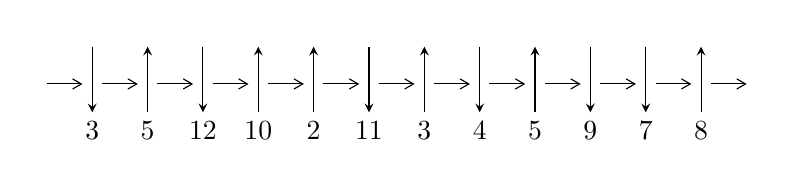
\begin{tikzpicture}[x=20pt, y=17pt]
	% nodes
	\node (C0) at (0, 0) {};
	\node (C1) at (1, 0) {};
	\node (C1U) at (1, +1) {};
	\node (C1D) at (1, -1) {3};

	\node (C2) at (2, 0) {};
	\node (C2U) at (2, +1) {};
	\node (C2D) at (2, -1) {5};

	\node (C3) at (3, 0) {};
	\node (C3U) at (3, +1) {};
	\node (C3D) at (3, -1) {12};

	\node (C4) at (4, 0) {};
	\node (C4U) at (4, +1) {};
	\node (C4D) at (4, -1) {10};

	\node (C5) at (5, 0) {};
	\node (C5U) at (5, +1) {};
	\node (C5D) at (5, -1) {2};

	\node (C6) at (6, 0) {};
	\node (C6U) at (6, +1) {};
	\node (C6D) at (6, -1) {11};

	\node (C7) at (7, 0) {};
	\node (C7U) at (7, +1) {};
	\node (C7D) at (7, -1) {3};

	\node (C8) at (8, 0) {};
	\node (C8U) at (8, +1) {};
	\node (C8D) at (8, -1) {4};

	\node (C9) at (9, 0) {};
	\node (C9U) at (9, +1) {};
	\node (C9D) at (9, -1) {5};

	\node (C10) at (10, 0) {};
	\node (C10U) at (10, +1) {};
	\node (C10D) at (10, -1) {9};

	\node (C11) at (11, 0) {};
	\node (C11U) at (11, +1) {};
	\node (C11D) at (11, -1) {7};

	\node (C12) at (12, 0) {};
	\node (C12U) at (12, +1) {};
	\node (C12D) at (12, -1) {8};
	\node (C13) at (13, 0) {};

	% arrows
	\draw[->,>={angle 60}]
	(C0) edge (C1) (C1) edge (C2) (C2) edge (C3) (C3) edge (C4) (C4) edge (C5) (C5) edge (C6) (C6) edge (C7) (C7) edge (C8) (C8) edge (C9) (C9) edge (C10) (C10) edge (C11) (C11) edge (C12) (C12) edge (C13) ;	\draw[->,>=stealth]
	(C1U) edge (C1D) (C2D) edge (C2U) (C3U) edge (C3D) (C4D) edge (C4U) (C5D) edge (C5U) (C6U) edge (C6D) (C7D) edge (C7U) (C8U) edge (C8D) (C9D) edge (C9U) (C10U) edge (C10D) (C11U) edge (C11D) (C12D) edge (C12U) ;
	\end{tikzpicture} \\
\hhline{~~} \\& 
\textbf{Solving Sequence} \\ \cline{2-2} 
 &
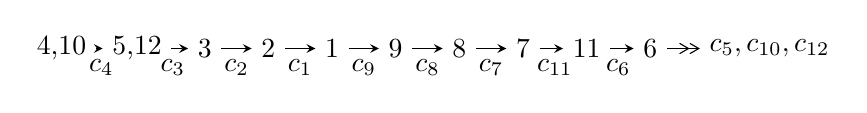
\begin{tikzpicture}[x=23pt, y=7pt]
	% node
	\node (A0) at (-1/8, 0) {4,10};
	\node (A1) at (17/16, 0) {5,12};
	\node (A2) at (17/8, 0) {3};
	\node (A3) at (25/8, 0) {2};
	\node (A4) at (33/8, 0) {1};
	\node (A5) at (41/8, 0) {9};
	\node (A6) at (49/8, 0) {8};
	\node (A7) at (57/8, 0) {7};
	\node (A8) at (65/8, 0) {11};
	\node (A9) at (73/8, 0) {6};
	\node (C1) at (1/2, -1) {$c_{4}$};
	\node (C2) at (13/8, -1) {$c_{3}$};
	\node (C3) at (21/8, -1) {$c_{2}$};
	\node (C4) at (29/8, -1) {$c_{1}$};
	\node (C5) at (37/8, -1) {$c_{9}$};
	\node (C6) at (45/8, -1) {$c_{8}$};
	\node (C7) at (53/8, -1) {$c_{7}$};
	\node (C8) at (61/8, -1) {$c_{11}$};
	\node (C9) at (69/8, -1) {$c_{6}$};
	\node (A10) at (11, 0) {$c_{5},c_{10},c_{12}$};

	% edge
	\draw[->,>=stealth]	
	(A0) edge (A1) (A1) edge (A2) (A2) edge (A3) (A3) edge (A4) (A4) edge (A5) (A5) edge (A6) (A6) edge (A7) (A7) edge (A8) (A8) edge (A9) ;
	\draw[->>,>={angle 60}]	
	(A9) edge (A10);
\end{tikzpicture} \\ 

\end{tabular} \\

\footnotetext{
The image of knot diagram is generated by the software ``\textbf{Draw programme}" developed by Andrew Bartholomew(\url{http://www.layer8.co.uk/maths/draw/index.htm\#Running-draw}), where we modified some parts for our purpose(\url{https://github.com/CATsTAILs/LinksPainter}).
}\phantom \\ \newline 
\centering \textbf{Ideals for irreducible components\footnotemark of $X_{\text{par}}$} 
 
\begin{align*}
I^u_{1}&=\langle 
-3 u^{18}-24 u^{17}+\cdots+2 b-14,\;-11 u^{18}-95 u^{17}+\cdots+8 a-48,\;u^{19}+9 u^{18}+\cdots+44 u+8\rangle \\
I^u_{2}&=\langle 
2 u^{15}-2 u^{14}+9 u^{13}-7 u^{12}+19 u^{11}-14 u^{10}+23 u^9-16 u^8+16 u^7-12 u^6+7 u^5-4 u^4+4 u^3+b+2 u+1,\\
\phantom{I^u_{2}}&\phantom{= \langle  }u^{15}+2 u^{14}+\cdots+a+4,\\
\phantom{I^u_{2}}&\phantom{= \langle  }u^{16}- u^{15}+5 u^{14}-4 u^{13}+12 u^{12}-9 u^{11}+17 u^{10}-12 u^9+15 u^8-11 u^7+9 u^6-6 u^5+5 u^4-2 u^3+3 u^2+1\rangle \\
\\
\end{align*}
\raggedright * 2 irreducible components of $\dim_{\mathbb{C}}=0$, with total 35 representations.\\
\footnotetext{All coefficients of polynomials are rational numbers. But the coefficients are sometimes approximated in decimal forms when there is not enough margin.}
\newpage
\renewcommand{\arraystretch}{1}
\centering \section*{I. $I^u_{1}= \langle -3 u^{18}-24 u^{17}+\cdots+2 b-14,\;-11 u^{18}-95 u^{17}+\cdots+8 a-48,\;u^{19}+9 u^{18}+\cdots+44 u+8 \rangle$}
\flushleft \textbf{(i) Arc colorings}\\
\begin{tabular}{m{7pt} m{180pt} m{7pt} m{180pt} }
\flushright $a_{4}=$&$\begin{pmatrix}1\\0\end{pmatrix}$ \\
\flushright $a_{10}=$&$\begin{pmatrix}0\\u\end{pmatrix}$ \\
\flushright $a_{5}=$&$\begin{pmatrix}1\\- u^2\end{pmatrix}$ \\
\flushright $a_{12}=$&$\begin{pmatrix}\frac{11}{8} u^{18}+\frac{95}{8} u^{17}+\cdots+\frac{67}{2} u+6\\\frac{3}{2} u^{18}+12 u^{17}+\cdots+\frac{67}{2} u+7\end{pmatrix}$ \\
\flushright $a_{3}=$&$\begin{pmatrix}\frac{3}{8} u^{18}+\frac{21}{8} u^{17}+\cdots-\frac{73}{4} u-\frac{9}{2}\\\frac{1}{4} u^{18}+\frac{5}{4} u^{17}+\cdots-9 u-1\end{pmatrix}$ \\
\flushright $a_{2}=$&$\begin{pmatrix}\frac{1}{8} u^{18}+\frac{3}{8} u^{17}+\cdots-\frac{157}{4} u-\frac{19}{2}\\\frac{1}{4} u^{18}+\frac{5}{4} u^{17}+\cdots-11 u-1\end{pmatrix}$ \\
\flushright $a_{1}=$&$\begin{pmatrix}\frac{3}{8} u^{18}+\frac{15}{8} u^{17}+\cdots-\frac{85}{2} u-10\\- u^{18}-\frac{19}{2} u^{17}+\cdots-\frac{131}{2} u-13\end{pmatrix}$ \\
\flushright $a_{9}=$&$\begin{pmatrix}- u\\u^3+u\end{pmatrix}$ \\
\flushright $a_{8}=$&$\begin{pmatrix}u^3\\u^3+u\end{pmatrix}$ \\
\flushright $a_{7}=$&$\begin{pmatrix}\frac{1}{8} u^{18}+\frac{11}{8} u^{17}+\cdots+\frac{31}{4} u+1\\-\frac{1}{4} u^{18}-\frac{7}{4} u^{17}+\cdots-\frac{23}{2} u-3\end{pmatrix}$ \\
\flushright $a_{11}=$&$\begin{pmatrix}- u^3\\u^5+u^3+u\end{pmatrix}$ \\
\flushright $a_{6}=$&$\begin{pmatrix}-\frac{7}{8} u^{18}-\frac{61}{8} u^{17}+\cdots-\frac{129}{4} u-7\\\frac{1}{4} u^{18}+\frac{7}{4} u^{17}+\cdots+\frac{57}{2} u+7\end{pmatrix}$\\&\end{tabular}
\flushleft \textbf{(ii) Obstruction class $= -1$}\\~\\
\flushleft \textbf{(iii) Cusp Shapes $= -8 u^{18}-66 u^{17}-305 u^{16}-975 u^{15}-2367 u^{14}-4600 u^{13}-7383 u^{12}-10049 u^{11}-11804 u^{10}-12134 u^9-11000 u^8-8792 u^7-6229 u^6-3932 u^5-2281 u^4-1230 u^3-584 u^2-212 u-42$}\\~\\
\newpage\renewcommand{\arraystretch}{1}
\flushleft \textbf{(iv) u-Polynomials at the component}\newline \\
\begin{tabular}{m{50pt}|m{274pt}}
Crossings & \hspace{64pt}u-Polynomials at each crossing \\
\hline $$\begin{aligned}c_{1}\end{aligned}$$&$\begin{aligned}
&u^{19}+50 u^{18}+\cdots+9 u-1
\end{aligned}$\\
\hline $$\begin{aligned}c_{2},c_{5},c_{7}\end{aligned}$$&$\begin{aligned}
&u^{19}+25 u^{17}+\cdots- u+1
\end{aligned}$\\
\hline $$\begin{aligned}c_{3}\end{aligned}$$&$\begin{aligned}
&u^{19}-4 u^{18}+\cdots+5 u-1
\end{aligned}$\\
\hline $$\begin{aligned}c_{4},c_{9}\end{aligned}$$&$\begin{aligned}
&u^{19}+9 u^{18}+\cdots+44 u+8
\end{aligned}$\\
\hline $$\begin{aligned}c_{6},c_{11}\end{aligned}$$&$\begin{aligned}
&u^{19}+3 u^{18}+\cdots+28 u^2+1
\end{aligned}$\\
\hline $$\begin{aligned}c_{8}\end{aligned}$$&$\begin{aligned}
&u^{19}-9 u^{18}+\cdots-4116 u+1960
\end{aligned}$\\
\hline $$\begin{aligned}c_{10}\end{aligned}$$&$\begin{aligned}
&u^{19}+9 u^{18}+\cdots-112 u-64
\end{aligned}$\\
\hline $$\begin{aligned}c_{12}\end{aligned}$$&$\begin{aligned}
&u^{19}- u^{18}+\cdots-104 u+193
\end{aligned}$\\
\hline
\end{tabular}\\~\\
\newpage\renewcommand{\arraystretch}{1}
\flushleft \textbf{(v) Riley Polynomials at the component}\newline \\
\begin{tabular}{m{50pt}|m{274pt}}
Crossings & \hspace{64pt}Riley Polynomials at each crossing \\
\hline $$\begin{aligned}c_{1}\end{aligned}$$&$\begin{aligned}
&y^{19}-202 y^{18}+\cdots+101 y-1
\end{aligned}$\\
\hline $$\begin{aligned}c_{2},c_{5},c_{7}\end{aligned}$$&$\begin{aligned}
&y^{19}+50 y^{18}+\cdots+9 y-1
\end{aligned}$\\
\hline $$\begin{aligned}c_{3}\end{aligned}$$&$\begin{aligned}
&y^{19}-2 y^{18}+\cdots+y-1
\end{aligned}$\\
\hline $$\begin{aligned}c_{4},c_{9}\end{aligned}$$&$\begin{aligned}
&y^{19}+9 y^{18}+\cdots-112 y-64
\end{aligned}$\\
\hline $$\begin{aligned}c_{6},c_{11}\end{aligned}$$&$\begin{aligned}
&y^{19}-49 y^{18}+\cdots-56 y-1
\end{aligned}$\\
\hline $$\begin{aligned}c_{8}\end{aligned}$$&$\begin{aligned}
&y^{19}-91 y^{18}+\cdots+10638096 y-3841600
\end{aligned}$\\
\hline $$\begin{aligned}c_{10}\end{aligned}$$&$\begin{aligned}
&y^{19}+y^{18}+\cdots-35584 y-4096
\end{aligned}$\\
\hline $$\begin{aligned}c_{12}\end{aligned}$$&$\begin{aligned}
&y^{19}+57 y^{18}+\cdots+85314 y-37249
\end{aligned}$\\
\hline
\end{tabular}\\~\\
\newpage\flushleft \textbf{(vi) Complex Volumes and Cusp Shapes}
$$\begin{array}{c|c|c}  
\text{Solutions to }I^u_{1}& \I (\text{vol} + \sqrt{-1}CS) & \text{Cusp shape}\\
 \hline 
\begin{aligned}
u &= \phantom{-}0.346161 + 0.956386 I \\
a &= \phantom{-}1.46736 + 0.28036 I \\
b &= \phantom{-}0.418807 - 0.392483 I\end{aligned}
 & -0.63169 + 2.23536 I & \phantom{-}1.18472 - 3.58566 I \\ \hline\begin{aligned}
u &= \phantom{-}0.346161 - 0.956386 I \\
a &= \phantom{-}1.46736 - 0.28036 I \\
b &= \phantom{-}0.418807 + 0.392483 I\end{aligned}
 & -0.63169 - 2.23536 I & \phantom{-}1.18472 + 3.58566 I \\ \hline\begin{aligned}
u &= -0.302273 + 1.061440 I \\
a &= -1.21082 + 0.86313 I \\
b &= -1.020080 + 0.439454 I\end{aligned}
 & -3.68086 - 0.50062 I & -7.63466 + 1.65999 I \\ \hline\begin{aligned}
u &= -0.302273 - 1.061440 I \\
a &= -1.21082 - 0.86313 I \\
b &= -1.020080 - 0.439454 I\end{aligned}
 & -3.68086 + 0.50062 I & -7.63466 - 1.65999 I \\ \hline\begin{aligned}
u &= -0.800161\phantom{ +0.000000I} \\
a &= \phantom{-}1.21345\phantom{ +0.000000I} \\
b &= \phantom{-}0.717995\phantom{ +0.000000I}\end{aligned}
 & -3.42695\phantom{ +0.000000I} & -3.98880\phantom{ +0.000000I} \\ \hline\begin{aligned}
u &= -0.536472 + 1.088430 I \\
a &= -1.78211 + 0.61588 I \\
b &= -0.874784 - 0.944864 I\end{aligned}
 & -2.09426 - 6.57381 I & -0.65064 + 5.14701 I \\ \hline\begin{aligned}
u &= -0.536472 - 1.088430 I \\
a &= -1.78211 - 0.61588 I \\
b &= -0.874784 + 0.944864 I\end{aligned}
 & -2.09426 + 6.57381 I & -0.65064 - 5.14701 I \\ \hline\begin{aligned}
u &= -0.628002 + 0.338042 I \\
a &= \phantom{-}0.039501 - 0.508734 I \\
b &= -0.649313 + 0.779497 I\end{aligned}
 & \phantom{-}0.03067 + 1.98876 I & \phantom{-}2.15859 - 2.97799 I \\ \hline\begin{aligned}
u &= -0.628002 - 0.338042 I \\
a &= \phantom{-}0.039501 + 0.508734 I \\
b &= -0.649313 - 0.779497 I\end{aligned}
 & \phantom{-}0.03067 - 1.98876 I & \phantom{-}2.15859 + 2.97799 I \\ \hline\begin{aligned}
u &= -0.455443 + 1.212920 I \\
a &= \phantom{-}1.89609 - 0.58745 I \\
b &= \phantom{-}0.758353 + 0.039269 I\end{aligned}
 & -6.99596 - 4.49122 I & -9.18387 - 0.01438 I\\
 \hline 
 \end{array}$$\newpage$$\begin{array}{c|c|c}  
\text{Solutions to }I^u_{1}& \I (\text{vol} + \sqrt{-1}CS) & \text{Cusp shape}\\
 \hline 
\begin{aligned}
u &= -0.455443 - 1.212920 I \\
a &= \phantom{-}1.89609 + 0.58745 I \\
b &= \phantom{-}0.758353 - 0.039269 I\end{aligned}
 & -6.99596 + 4.49122 I & -9.18387 + 0.01438 I \\ \hline\begin{aligned}
u &= \phantom{-}0.413988 + 0.520782 I \\
a &= \phantom{-}0.288663 - 0.426959 I \\
b &= -0.084685 + 0.588329 I\end{aligned}
 & \phantom{-}0.657337 + 1.088170 I & \phantom{-}4.45180 - 5.21852 I \\ \hline\begin{aligned}
u &= \phantom{-}0.413988 - 0.520782 I \\
a &= \phantom{-}0.288663 + 0.426959 I \\
b &= -0.084685 - 0.588329 I\end{aligned}
 & \phantom{-}0.657337 - 1.088170 I & \phantom{-}4.45180 + 5.21852 I \\ \hline\begin{aligned}
u &= -1.41615 + 0.03594 I \\
a &= \phantom{-}0.802995 - 0.190440 I \\
b &= \phantom{-}1.04189 + 1.04688 I\end{aligned}
 & \phantom{-}18.3876 - 3.8412 I & -1.79058 + 1.95309 I \\ \hline\begin{aligned}
u &= -1.41615 - 0.03594 I \\
a &= \phantom{-}0.802995 + 0.190440 I \\
b &= \phantom{-}1.04189 - 1.04688 I\end{aligned}
 & \phantom{-}18.3876 + 3.8412 I & -1.79058 - 1.95309 I \\ \hline\begin{aligned}
u &= -0.78204 + 1.42833 I \\
a &= \phantom{-}0.573067 - 0.779029 I \\
b &= \phantom{-}0.97983 - 1.07686 I\end{aligned}
 & \phantom{-}14.2330 - 3.7497 I & -3.12835 + 0.88970 I \\ \hline\begin{aligned}
u &= -0.78204 - 1.42833 I \\
a &= \phantom{-}0.573067 + 0.779029 I \\
b &= \phantom{-}0.97983 + 1.07686 I\end{aligned}
 & \phantom{-}14.2330 + 3.7497 I & -3.12835 - 0.88970 I \\ \hline\begin{aligned}
u &= -0.73969 + 1.46029 I \\
a &= \phantom{-}1.81853 - 0.33078 I \\
b &= \phantom{-}1.07098 + 0.99229 I\end{aligned}
 & \phantom{-}13.8839 - 11.3207 I & -3.41262 + 4.66030 I \\ \hline\begin{aligned}
u &= -0.73969 - 1.46029 I \\
a &= \phantom{-}1.81853 + 0.33078 I \\
b &= \phantom{-}1.07098 - 0.99229 I\end{aligned}
 & \phantom{-}13.8839 + 11.3207 I & -3.41262 - 4.66030 I\\
 \hline 
 \end{array}$$\newpage\newpage\renewcommand{\arraystretch}{1}
\centering \section*{II. $I^u_{2}= \langle 2 u^{15}-2 u^{14}+\cdots+b+1,\;u^{15}+2 u^{14}+\cdots+a+4,\;u^{16}- u^{15}+\cdots+3 u^2+1 \rangle$}
\flushleft \textbf{(i) Arc colorings}\\
\begin{tabular}{m{7pt} m{180pt} m{7pt} m{180pt} }
\flushright $a_{4}=$&$\begin{pmatrix}1\\0\end{pmatrix}$ \\
\flushright $a_{10}=$&$\begin{pmatrix}0\\u\end{pmatrix}$ \\
\flushright $a_{5}=$&$\begin{pmatrix}1\\- u^2\end{pmatrix}$ \\
\flushright $a_{12}=$&$\begin{pmatrix}- u^{15}-2 u^{14}+\cdots+u-4\\-2 u^{15}+2 u^{14}+\cdots-2 u-1\end{pmatrix}$ \\
\flushright $a_{3}=$&$\begin{pmatrix}- u^{15}-2 u^{13}+\cdots+u-3\\-2 u^{15}+3 u^{14}+\cdots-2 u-1\end{pmatrix}$ \\
\flushright $a_{2}=$&$\begin{pmatrix}- u^{15}- u^{13}+\cdots+2 u-3\\-3 u^{15}+4 u^{14}+\cdots-2 u-1\end{pmatrix}$ \\
\flushright $a_{1}=$&$\begin{pmatrix}- u^{15}- u^{14}+\cdots+2 u-3\\-3 u^{15}+3 u^{14}+\cdots-2 u-1\end{pmatrix}$ \\
\flushright $a_{9}=$&$\begin{pmatrix}- u\\u^3+u\end{pmatrix}$ \\
\flushright $a_{8}=$&$\begin{pmatrix}u^3\\u^3+u\end{pmatrix}$ \\
\flushright $a_{7}=$&$\begin{pmatrix}u^{14}-2 u^{13}+\cdots-3 u+1\\u^{15}- u^{14}+\cdots+u+1\end{pmatrix}$ \\
\flushright $a_{11}=$&$\begin{pmatrix}- u^3\\u^5+u^3+u\end{pmatrix}$ \\
\flushright $a_{6}=$&$\begin{pmatrix}2 u^{14}-3 u^{13}+\cdots-3 u+2\\u^{15}+3 u^{13}+\cdots+2 u^2+2\end{pmatrix}$\\&\end{tabular}
\flushleft \textbf{(ii) Obstruction class $= 1$}\\~\\
\flushleft \textbf{(iii) Cusp Shapes $= 8 u^{15}-8 u^{14}+36 u^{13}-27 u^{12}+74 u^{11}-55 u^{10}+90 u^9-67 u^8+63 u^7-54 u^6+32 u^5-18 u^4+16 u^3+3 u^2+10 u-3$}\\~\\
\newpage\renewcommand{\arraystretch}{1}
\flushleft \textbf{(iv) u-Polynomials at the component}\newline \\
\begin{tabular}{m{50pt}|m{274pt}}
Crossings & \hspace{64pt}u-Polynomials at each crossing \\
\hline $$\begin{aligned}c_{1}\end{aligned}$$&$\begin{aligned}
&u^{16}-11 u^{15}+\cdots-9 u+1
\end{aligned}$\\
\hline $$\begin{aligned}c_{2},c_{7}\end{aligned}$$&$\begin{aligned}
&u^{16}- u^{15}+\cdots- u+1
\end{aligned}$\\
\hline $$\begin{aligned}c_{3}\end{aligned}$$&$\begin{aligned}
&u^{16}+7 u^{15}+\cdots+5 u+1
\end{aligned}$\\
\hline $$\begin{aligned}c_{4}\end{aligned}$$&$\begin{aligned}
&u^{16}- u^{15}+\cdots+3 u^2+1
\end{aligned}$\\
\hline $$\begin{aligned}c_{5}\end{aligned}$$&$\begin{aligned}
&u^{16}+u^{15}+\cdots+u+1
\end{aligned}$\\
\hline $$\begin{aligned}c_{6}\end{aligned}$$&$\begin{aligned}
&u^{16}+2 u^{15}+\cdots+2 u+1
\end{aligned}$\\
\hline $$\begin{aligned}c_{8}\end{aligned}$$&$\begin{aligned}
&u^{16}- u^{15}+\cdots+4 u^2+1
\end{aligned}$\\
\hline $$\begin{aligned}c_{9}\end{aligned}$$&$\begin{aligned}
&u^{16}+u^{15}+\cdots+3 u^2+1
\end{aligned}$\\
\hline $$\begin{aligned}c_{10}\end{aligned}$$&$\begin{aligned}
&u^{16}+9 u^{15}+\cdots+6 u+1
\end{aligned}$\\
\hline $$\begin{aligned}c_{11}\end{aligned}$$&$\begin{aligned}
&u^{16}-2 u^{15}+\cdots-2 u+1
\end{aligned}$\\
\hline $$\begin{aligned}c_{12}\end{aligned}$$&$\begin{aligned}
&u^{16}+7 u^{14}+\cdots+4 u^2+1
\end{aligned}$\\
\hline
\end{tabular}\\~\\
\newpage\renewcommand{\arraystretch}{1}
\flushleft \textbf{(v) Riley Polynomials at the component}\newline \\
\begin{tabular}{m{50pt}|m{274pt}}
Crossings & \hspace{64pt}Riley Polynomials at each crossing \\
\hline $$\begin{aligned}c_{1}\end{aligned}$$&$\begin{aligned}
&y^{16}-5 y^{15}+\cdots+5 y+1
\end{aligned}$\\
\hline $$\begin{aligned}c_{2},c_{5},c_{7}\end{aligned}$$&$\begin{aligned}
&y^{16}+11 y^{15}+\cdots+9 y+1
\end{aligned}$\\
\hline $$\begin{aligned}c_{3}\end{aligned}$$&$\begin{aligned}
&y^{16}- y^{15}+\cdots+y+1
\end{aligned}$\\
\hline $$\begin{aligned}c_{4},c_{9}\end{aligned}$$&$\begin{aligned}
&y^{16}+9 y^{15}+\cdots+6 y+1
\end{aligned}$\\
\hline $$\begin{aligned}c_{6},c_{11}\end{aligned}$$&$\begin{aligned}
&y^{16}-12 y^{15}+\cdots-6 y+1
\end{aligned}$\\
\hline $$\begin{aligned}c_{8}\end{aligned}$$&$\begin{aligned}
&y^{16}-7 y^{15}+\cdots+8 y+1
\end{aligned}$\\
\hline $$\begin{aligned}c_{10}\end{aligned}$$&$\begin{aligned}
&y^{16}+y^{15}+\cdots+2 y+1
\end{aligned}$\\
\hline $$\begin{aligned}c_{12}\end{aligned}$$&$\begin{aligned}
&y^{16}+14 y^{15}+\cdots+8 y+1
\end{aligned}$\\
\hline
\end{tabular}\\~\\
\newpage\flushleft \textbf{(vi) Complex Volumes and Cusp Shapes}
$$\begin{array}{c|c|c}  
\text{Solutions to }I^u_{2}& \I (\text{vol} + \sqrt{-1}CS) & \text{Cusp shape}\\
 \hline 
\begin{aligned}
u &= \phantom{-}0.335104 + 0.911069 I \\
a &= \phantom{-}2.45662 - 0.85727 I \\
b &= \phantom{-}0.921522 + 0.158810 I\end{aligned}
 & -7.02394 + 1.39379 I & -9.47279 + 0.73629 I \\ \hline\begin{aligned}
u &= \phantom{-}0.335104 - 0.911069 I \\
a &= \phantom{-}2.45662 + 0.85727 I \\
b &= \phantom{-}0.921522 - 0.158810 I\end{aligned}
 & -7.02394 - 1.39379 I & -9.47279 - 0.73629 I \\ \hline\begin{aligned}
u &= -0.379248 + 1.028620 I \\
a &= -0.646901 + 1.136830 I \\
b &= -1.14774 + 0.83032 I\end{aligned}
 & -3.77746 + 0.63307 I & -8.74418 - 3.43739 I \\ \hline\begin{aligned}
u &= -0.379248 - 1.028620 I \\
a &= -0.646901 - 1.136830 I \\
b &= -1.14774 - 0.83032 I\end{aligned}
 & -3.77746 - 0.63307 I & -8.74418 + 3.43739 I \\ \hline\begin{aligned}
u &= \phantom{-}0.814712 + 0.313052 I \\
a &= -0.637439 + 0.085695 I \\
b &= -0.219047 + 0.658555 I\end{aligned}
 & -2.04483 + 1.12270 I & \phantom{-}0.01080 - 2.10787 I \\ \hline\begin{aligned}
u &= \phantom{-}0.814712 - 0.313052 I \\
a &= -0.637439 - 0.085695 I \\
b &= -0.219047 - 0.658555 I\end{aligned}
 & -2.04483 - 1.12270 I & \phantom{-}0.01080 + 2.10787 I \\ \hline\begin{aligned}
u &= -0.532348 + 1.055360 I \\
a &= -1.92201 + 0.51905 I \\
b &= -0.99317 - 1.17536 I\end{aligned}
 & -2.65168 - 7.12816 I & -8.0544 + 12.2171 I \\ \hline\begin{aligned}
u &= -0.532348 - 1.055360 I \\
a &= -1.92201 - 0.51905 I \\
b &= -0.99317 + 1.17536 I\end{aligned}
 & -2.65168 + 7.12816 I & -8.0544 - 12.2171 I \\ \hline\begin{aligned}
u &= -0.569437 + 0.482937 I \\
a &= \phantom{-}0.475047 + 0.043194 I \\
b &= -0.782251 + 1.053490 I\end{aligned}
 & -0.93348 + 2.66812 I & -2.81990 - 6.15304 I \\ \hline\begin{aligned}
u &= -0.569437 - 0.482937 I \\
a &= \phantom{-}0.475047 - 0.043194 I \\
b &= -0.782251 - 1.053490 I\end{aligned}
 & -0.93348 - 2.66812 I & -2.81990 + 6.15304 I\\
 \hline 
 \end{array}$$\newpage$$\begin{array}{c|c|c}  
\text{Solutions to }I^u_{2}& \I (\text{vol} + \sqrt{-1}CS) & \text{Cusp shape}\\
 \hline 
\begin{aligned}
u &= -0.182107 + 0.721236 I \\
a &= -2.18930 + 1.30740 I \\
b &= -0.958246 - 0.624440 I\end{aligned}
 & -2.38549 - 3.31503 I & -6.02251 + 3.66103 I \\ \hline\begin{aligned}
u &= -0.182107 - 0.721236 I \\
a &= -2.18930 - 1.30740 I \\
b &= -0.958246 + 0.624440 I\end{aligned}
 & -2.38549 + 3.31503 I & -6.02251 - 3.66103 I \\ \hline\begin{aligned}
u &= \phantom{-}0.614974 + 1.102350 I \\
a &= \phantom{-}0.301915 + 0.157095 I \\
b &= \phantom{-}0.241401 - 0.693802 I\end{aligned}
 & -4.28291 + 4.20394 I & -2.40515 - 3.76480 I \\ \hline\begin{aligned}
u &= \phantom{-}0.614974 - 1.102350 I \\
a &= \phantom{-}0.301915 - 0.157095 I \\
b &= \phantom{-}0.241401 + 0.693802 I\end{aligned}
 & -4.28291 - 4.20394 I & -2.40515 + 3.76480 I \\ \hline\begin{aligned}
u &= \phantom{-}0.398350 + 1.236570 I \\
a &= -1.83794 + 0.04383 I \\
b &= -0.562464 + 0.307777 I\end{aligned}
 & -6.50903 + 5.01414 I & -1.49188 - 7.53690 I \\ \hline\begin{aligned}
u &= \phantom{-}0.398350 - 1.236570 I \\
a &= -1.83794 - 0.04383 I \\
b &= -0.562464 - 0.307777 I\end{aligned}
 & -6.50903 - 5.01414 I & -1.49188 + 7.53690 I\\
 \hline 
 \end{array}$$\newpage
\newpage\renewcommand{\arraystretch}{1}
\centering \section*{ III. u-Polynomials}
\begin{tabular}{m{50pt}|m{274pt}}
Crossings & \hspace{64pt}u-Polynomials at each crossing \\
\hline $$\begin{aligned}c_{1}\end{aligned}$$&$\begin{aligned}
&(u^{16}-11 u^{15}+\cdots-9 u+1)(u^{19}+50 u^{18}+\cdots+9 u-1)
\end{aligned}$\\
\hline $$\begin{aligned}c_{2},c_{7}\end{aligned}$$&$\begin{aligned}
&(u^{16}- u^{15}+\cdots- u+1)(u^{19}+25 u^{17}+\cdots- u+1)
\end{aligned}$\\
\hline $$\begin{aligned}c_{3}\end{aligned}$$&$\begin{aligned}
&(u^{16}+7 u^{15}+\cdots+5 u+1)(u^{19}-4 u^{18}+\cdots+5 u-1)
\end{aligned}$\\
\hline $$\begin{aligned}c_{4}\end{aligned}$$&$\begin{aligned}
&(u^{16}- u^{15}+\cdots+3 u^2+1)(u^{19}+9 u^{18}+\cdots+44 u+8)
\end{aligned}$\\
\hline $$\begin{aligned}c_{5}\end{aligned}$$&$\begin{aligned}
&(u^{16}+u^{15}+\cdots+u+1)(u^{19}+25 u^{17}+\cdots- u+1)
\end{aligned}$\\
\hline $$\begin{aligned}c_{6}\end{aligned}$$&$\begin{aligned}
&(u^{16}+2 u^{15}+\cdots+2 u+1)(u^{19}+3 u^{18}+\cdots+28 u^2+1)
\end{aligned}$\\
\hline $$\begin{aligned}c_{8}\end{aligned}$$&$\begin{aligned}
&(u^{16}- u^{15}+\cdots+4 u^2+1)(u^{19}-9 u^{18}+\cdots-4116 u+1960)
\end{aligned}$\\
\hline $$\begin{aligned}c_{9}\end{aligned}$$&$\begin{aligned}
&(u^{16}+u^{15}+\cdots+3 u^2+1)(u^{19}+9 u^{18}+\cdots+44 u+8)
\end{aligned}$\\
\hline $$\begin{aligned}c_{10}\end{aligned}$$&$\begin{aligned}
&(u^{16}+9 u^{15}+\cdots+6 u+1)(u^{19}+9 u^{18}+\cdots-112 u-64)
\end{aligned}$\\
\hline $$\begin{aligned}c_{11}\end{aligned}$$&$\begin{aligned}
&(u^{16}-2 u^{15}+\cdots-2 u+1)(u^{19}+3 u^{18}+\cdots+28 u^2+1)
\end{aligned}$\\
\hline $$\begin{aligned}c_{12}\end{aligned}$$&$\begin{aligned}
&(u^{16}+7 u^{14}+\cdots+4 u^2+1)(u^{19}- u^{18}+\cdots-104 u+193)
\end{aligned}$\\
\hline
\end{tabular}\newpage\renewcommand{\arraystretch}{1}
\centering \section*{ IV. Riley Polynomials}
\begin{tabular}{m{50pt}|m{274pt}}
Crossings & \hspace{64pt}Riley Polynomials at each crossing \\
\hline $$\begin{aligned}c_{1}\end{aligned}$$&$\begin{aligned}
&(y^{16}-5 y^{15}+\cdots+5 y+1)(y^{19}-202 y^{18}+\cdots+101 y-1)
\end{aligned}$\\
\hline $$\begin{aligned}c_{2},c_{5},c_{7}\end{aligned}$$&$\begin{aligned}
&(y^{16}+11 y^{15}+\cdots+9 y+1)(y^{19}+50 y^{18}+\cdots+9 y-1)
\end{aligned}$\\
\hline $$\begin{aligned}c_{3}\end{aligned}$$&$\begin{aligned}
&(y^{16}- y^{15}+\cdots+y+1)(y^{19}-2 y^{18}+\cdots+y-1)
\end{aligned}$\\
\hline $$\begin{aligned}c_{4},c_{9}\end{aligned}$$&$\begin{aligned}
&(y^{16}+9 y^{15}+\cdots+6 y+1)(y^{19}+9 y^{18}+\cdots-112 y-64)
\end{aligned}$\\
\hline $$\begin{aligned}c_{6},c_{11}\end{aligned}$$&$\begin{aligned}
&(y^{16}-12 y^{15}+\cdots-6 y+1)(y^{19}-49 y^{18}+\cdots-56 y-1)
\end{aligned}$\\
\hline $$\begin{aligned}c_{8}\end{aligned}$$&$\begin{aligned}
&(y^{16}-7 y^{15}+\cdots+8 y+1)\\
&\cdot(y^{19}-91 y^{18}+\cdots+10638096 y-3841600)
\end{aligned}$\\
\hline $$\begin{aligned}c_{10}\end{aligned}$$&$\begin{aligned}
&(y^{16}+y^{15}+\cdots+2 y+1)(y^{19}+y^{18}+\cdots-35584 y-4096)
\end{aligned}$\\
\hline $$\begin{aligned}c_{12}\end{aligned}$$&$\begin{aligned}
&(y^{16}+14 y^{15}+\cdots+8 y+1)(y^{19}+57 y^{18}+\cdots+85314 y-37249)
\end{aligned}$\\
\hline
\end{tabular}
\vskip 2pc
\end{document}